\documentclass[11pt]{article}
%\usepackage{fullpage}
\usepackage[top=2cm, bottom=1.5cm, left=1.5cm, right=1.5cm]{geometry}
\usepackage{amsmath,amsthm,amsfonts,amssymb,amscd}
\usepackage{xcolor}
\usepackage{graphicx}
\usepackage[utf8]{inputenc}
\usepackage[english]{babel}
\usepackage{fancyhdr}
\usepackage{wrapfig}

\pagestyle{fancy}
\fancyhf{}
\fancyhead[LO]{Mechanics \& Relativity F3210}
\fancyhead[RO]{Workshop 6: Energy \& Momentum}
%\fancyfoot[CE,CO]{\leftmark}
%\fancyfoot[LE,RO]{\thepage}

%answers
\usepackage{etoolbox}
\providetoggle{answers}
\settoggle{answers}{false}

\newcommand\vect[1]{\underline{\mathbf{#1}}}
\newcommand\unitvect[1]{\hat{\boldsymbol{#1}}}

\begin{document}

\noindent
\textbf{\textcolor{red}{Please upload your solution to Problem 3 to canvas for marking after the workshop.}}\\

\section*{Problem 1}

A 1.50 kg snowball is fired from a cliff 12.5 m high. The snowball?s initial velocity is 14.0 ms$^{-1}$, directed 41.0$^{\circ}$ above the horizontal. \\
(a) How much work is done on the snowball by the gravitational force during its flight to the flat ground below the cliff?\\
(b) What is the change in the gravitational potential energy of the snowball?Earth system during the flight? \\
(c) If that gravitational potential energy is taken to be zero at the height of the cliff, what is its value when the snowball reaches the ground?\\


\noindent

\section*{Problem 2}
A particle can slide along a track with elevated ends and a flat central part, as shown in the figure below. The flat part has length $L = 40$~cm. The curved portions of the track are frictionless, but for the flat part the coefficient of kinetic friction is $\mu_k = 0.20$. The particle is released from rest at point A, which is at height $h = L/2$. How far from the left edge of the flat part does the particle finally stop?

\begin{figure}[h]
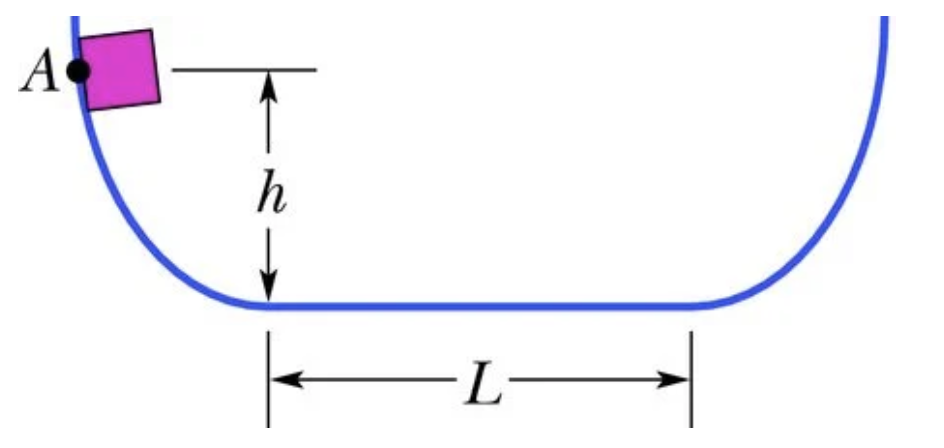
\includegraphics[scale=0.5]{2021-W6-Q2}

\end{figure}

\section*{\textcolor{red}{Problem 3}}
\fbox{\begin{minipage}{\textwidth}

A uniform can of mass 0.140 kg is 12.0 cm tall and filled with 0.354 kg of liquid. Then small holes are drilled in the top and bottom (with negligible loss of metal) to drain the liquid. \\
 (a) What is the initial height $h_i$ of the centre-of-mass of the can and contents?\\
 (b) What is the final height $h_f$ after the can loses all the liquid? \\
 (c) What is the height of the remaining liquid when the centre-of-mass reaches its lowest point?

\end{minipage}}


\section*{Problem 4}
A 4.0 kg mess kit sliding on a frictionless surface explodes into two 2.0 kg parts: 3.0 ms$^{-1}$, due north, and 5.0 ms$^{-1}$, 30$^{\circ}$ north of east. What is the original speed of the mess kit?


%\vspace{0.5cm}
\section*{Want more practice?}
\small
Further problems on PE: Chapter 8.1-8.3 \\
Further problems on Cos of E: Chapter 8.4-8.5 \\
Further problems on CofM and linear momentum: Chapter 9\\
\end{document}





 




 


